\section{Dispersion relations for concrete graph topologies} \label{sec:ScalarExamples}
In this section we provide examples to demonstrate how the spectrum of the problem \eqref{eq:WholeSpaceLaplaceEqn} is obtained via the analysis of the $M$-matrix for the quantum graph problem \eqref{eq:QGFullSystem}.
The examples are chosen to highlight the methodology and some of the remarks discussed in sections \ref{sec:QuantumGraphs} and \ref{sec:Discussion}, and to motivate the final discussion in section \ref{sec:Conclusion}. 

\subsection{One-Dimensional Loop} \label{ssec:Example1DLoop}
We begin with the simplest example: a ``chain" of vertices that is periodic in one direction, to demonstrate how one takes the period graph of a physical singular-structure and employs proposition \ref{prop:M-MatrixEntries} to construct the $M$-matrix and extract the spectral information.
We also highlight the necessity of ``splitting" edges of a graph via the use of ``dummy vertices", to remove loops and edge-lengths that are rationally-related to compliment section \ref{ssec:ArtificialVertices}.

Consider the graph $\graph$ periodic in one direction in $\reals\times\sqbracs{0,1}$, with vertices $v_j = \bracs{j + \recip{2}, 0}^\top$ and edges $I_{j\bracs{j+1}}, \ j\in\integers$.
Since $\graph$ is only periodic in the $x_1$-direction, the period cell lies in $S^1\times\sqbracs{0,1}$ rather than the 2D-torus, and the quasi-momentum $\qm\in\left[-\pi,\pi\right)$ is scalar (one can set $\qm_2=0$ in \eqref{eq:QGFullSystem} when constructing the $\qm_{jk}$ to account for the lack of periodicity in $x_2$).
Place identical coupling constants at each vertex, with $\alpha_j = \alpha_1 \ \forall j$.
The quantum graph that corresponds to the period graph of $\graph$ consists of a single vertex $v$ with a looping edge $I$ of length 1, with quasi-momentum $\qm$ on $I$ and coupling constant $\alpha_1$ at $v$.
We must introduce an artificial vertex (section \ref{ssec:ArtificialVertices}) to break the loop $I$ into two edges with irrationally-related edge lengths, producing a new quantum graph $\graph_{\mathcal{P}}=\bracs{\vertSet, \edgeSet}$ with
\begin{align*}
	\vertSet = \clbracs{ v_1 , v_2 }, \quad \edgeSet = \clbracs{ I_{12}, I_{21} },
	&\qquad \abs{I_{12}} = a, \quad \abs{I_{21}} = 1-a, \quad \qm_{12} = \qm_{21} = \qm, 
	&\qquad \alpha_1 >0, \quad &\alpha_2 = 0,
\end{align*}
where $a$ and $1-a$ are irrationally related --- taking $a = \recip{\sqrt{2}}$ would suffice, for example.
The process of moving from $\graph$ to $\graph_{\mathcal{P}}$ is illustrated in figure \ref{fig:Diagram_1DExample}.
Studying the $M$-matrix of $\graph_{\mathcal{P}}$ to determine the eigenvalues $\omega^2$ is now equivalent to studying the spectrum of the original problem.
\begin{figure}[b!]
	\centering
	\begin{subfigure}[t]{0.3\textwidth}
		\centering
		\includegraphics[scale=2]{Diagram_1DLineGraph.pdf}
		\caption{\label{fig:Diagram_1DLineGraph} The graph $\graph$, periodic in one dimension, consisting of integer-spaced vertices.}
	\end{subfigure}
	~
	\begin{subfigure}[t]{0.3\textwidth}
		\centering
		\includegraphics[scale=2]{Diagram_1DLineQuantumGraph.pdf}
		\caption{\label{fig:Diagram_1DLineQuantumGraph} The corresponding quantum graph of the period cell of $\graph$, containing one (looping) edge of length 1}
	\end{subfigure}
	~
	\begin{subfigure}[t]{0.3\textwidth}
		\centering
		\includegraphics[scale=2]{Diagram_1DLineComputationGraph.pdf}	
		\caption{\label{fig:Diagram_1DLineComputationGraph} The equivalent graph $\graph_{\mathcal{P}}$ that we study. Note that the dummy vertex $v_2$ has coupling constant 0.}
	\end{subfigure}
	\caption{\label{fig:Diagram_1DExample} The graphs $\graph$ and $\graph_{\mathcal{P}}$.}
\end{figure} \newline

Using proposition \ref{prop:M-MatrixEntries} and corollary \ref{cory:M-MatrixEntriesNoPoles}, and setting
\begin{align*}
	s_a\bracs{\omega} &= \sin\bracs{a\omega}, \quad c_a\bracs{\omega} = \cos\bracs{a\omega}, 
	\quad \tilde{s}_a\bracs{\omega} = \sin\bracs{(1-a)\omega}, \quad \tilde{c}_a\bracs{\omega} = \cos\bracs{(1-a)\omega},
\end{align*} 
we find that
\begin{align*}
	\mathfrak{M}_{\qm}\bracs{\omega^2} &= 
	\begin{pmatrix}[1.75]
		-\omega c_a \tilde{s}_a - \omega s_a \tilde{c}_{a} + \omega^2\alpha_1 s_a \tilde{s}_a &
		\omega e^{\rmi\qm a} \tilde{s}_a + \omega e^{-\rmi\qm(1-a)} s_a \\
		\omega e^{-\rmi\qm a} \tilde{s}_a + \omega e^{\rmi\qm(1-a)} s_a &
		-\omega c_a \tilde{s}_a - \omega s_a \tilde{c}_a
	\end{pmatrix}, \\
	H^{(2)}\bracs{\omega^2} &= s_a\bracs{\omega} s_b\bracs{\omega},\\
\end{align*}
where we have suppressed the dependencies on $\omega$ and $\omega^2$ for brevity --- we will only emphasise these dependencies in important formulae.
Computing $\det\mathfrak{M}_{\qm}\bracs{\omega^2}$ and solving \eqref{eq:QGDetSolveCondition} yields
\begin{align} \label{eq:1DChainDetEqual0}
	0 = 2\omega^2 s_a\bracs{\omega} \tilde{s}_a\bracs{\omega} \bracs{ \cos\omega - \frac{\omega\alpha_1}{2}\sin\omega - \cos\qm }.
\end{align}
Notice that the factor in front of the brackets in \eqref{eq:1DChainDetEqual0} is $2\omega^2 H^{(2)}\bracs{\omega^2}$, so is zero at $\omega=0$ and at the roots of $H^{(2)}$.
Otherwise, since $\cos\qm$ attains every value in $\sqbracs{-1,1}$ for $\qm\in\left[-\pi,\pi\right)$, the bracketed term in \eqref{eq:1DChainDetEqual0} implies that any $\omega$ satisfying
\begin{align*}
	-1 \leq \cos\omega - \frac{\omega\alpha_1}{2}\sin\omega \leq 1,
\end{align*}
is part of the spectrum of \eqref{eq:QGFullSystem}.

We now consider solutions of \eqref{eq:1DChainDetEqual0} that are also zeros of $H^{(2)}$ --- let $\omega_0$ denote one of these values, so $\omega_0\in\clbracs{\frac{n\pi}{a}, \frac{n\pi}{b} \setVert n\in\naturals }$.
The eigenvalue branches of $\mathfrak{M}_{\qm}$ can be computed,
\begin{align*}
	\widetilde{\beta}_{\pm, \qm}\bracs{\omega^2} &= -\omega\sin\omega + \frac{\omega^2\alpha_1}{2}s_a \tilde{s}_a \pm \omega\sqrt{ \sin^2\omega + \frac{\omega^2\alpha_1^2}{4}s_a^2 \tilde{s}_a^2 - 2s_a \tilde{s}_a\bracs{\cos\omega+\cos\qm} },
\end{align*}
however only $\widetilde{\beta}_{+, \qm}\bracs{\omega_0^2}=0$.
As such, $\omega_0$ is part of the spectrum of \eqref{eq:QGFullSystem} when
\begin{align*}
	\lim_{\omega\rightarrow\omega_0}\bracs{ H^{(2)}\bracs{\omega^2} }^{-1}\widetilde{\beta}\bracs{\omega^2}_{+} = 0,
\end{align*}
which (after applying L'h\^ospital's rule) only occurs when
\begin{align*}
	\exists\qm_0\in\left[-\pi,\pi\right) \text{ s.t. } \cos\omega_0 - \frac{\omega_0\alpha_1}{2}\sin\omega_0 - \cos\qm_0 = 0. 
\end{align*}
Therefore, the spectrum of \eqref{eq:QGFullSystem} is fully described by those $\omega$ that satisfy
\begin{align*}
	\-1 \leq \cos\omega - \frac{\omega\alpha_1}{2}\sin\omega \leq 1.
\end{align*}

Breaking the looping edge and ensuring that the resulting edge-lengths are irrationally-related is necessary to obtain a full description of the spectrum, and failure to do so results in the loss of the Dirichlet eigenvalues.
By way of illustration, if the looping edge is not broken then one obtains
\begin{align*}
	\det\mathfrak{M}_{\qm}\bracs{\omega^2} &= \cos\omega - \frac{\omega\alpha_1}{2}\sin\omega - \cos\qm, \\
	H^{(2)}\bracs{\omega^2} &= \omega\sin\omega, \\
	\beta_{\qm}\bracs{\omega^2} &= \cos\omega - \frac{\omega\alpha_1}{2}\sin\omega - \cos\qm.
\end{align*}
This means that $\beta_{0}\bracs{(2k\pi)^2}=0$ and $\beta_{-\pi}\bracs{(2(k-1)\pi)^2}=0$ for $k\in\naturals$, but 
\begin{align*}
	\lim_{\omega\rightarrow 2k\pi}H^{(2)}\bracs{\omega^2}\beta_{0}\bracs{\omega^2} &= \alpha_1\bracs{2k\pi}^2 \neq 0, \\
	\lim_{\omega\rightarrow 2(k-1)\pi} H^{(2)}\bracs{\omega^2}\beta_{-\pi}\bracs{\omega^2} &= \alpha_1\bracs{2(k-1)\pi}^2 \neq 0,
\end{align*}
which leads one to falsely exclude $\omega=n\pi, \ n\in\naturals$ from the spectrum.
These cases $\omega=2k\pi, \qm=0$ and $\omega=2(k-1)\pi, \qm=-\pi$ are in fact the eigenvalues of the problem
\begin{align*}
	-\bracs{\diff{}{t} + \rmi\qm_{jk}}^2 \tilde{u}_{jk} = \omega^2 \tilde{u}_{jk}, \quad &t\in\interval{I_{jk}}, \quad \forall I_{jk}\in \edgeSet, \\
	u \text{ is continuous at each } &v_j \in \vertSet, \\
	u\bracs{v_j} = 0, \quad &v_j\in\vertSet,
\end{align*}
which also happen to be solutions to \eqref{eq:QGFullSystem}.
Similar problems occur when the lengths $a$ and $1-a$ are rationally related --- taking $a=\recip{2}$ results in similar ``loss" of the eigenvalues $\omega=2k\pi, \ k\in\naturals$, for example.

\subsection{``Decorated" Graph with Dependencies Arising from the Embedding} \label{ssec:EmbeddingDependentExample}
We next provide an explicit example to complement the discussion that concluded section \ref{ssec:MMatrix}, concerning our decision to bestow our quantum graphs with an embedding. 
To avoid confusion in this section, the term ``quantum graph" will be prefixed with ``(embedded)" when we are discussing an quantum graph that has been equipped with an embedding, and prefixed with ``(abstract)" when referring to a quantum graph that has not been assigned an embedding.

Consider the (embedded) graph $\graph$ in $\reals\times\sqbracs{0,1}$, with vertices
\begin{align*}
	v_1^m = \bracs{m + \recip{2}, \recip{2}}^\top, 
	&\quad v_2^m = \bracs{m + \recip{2}\bracs{1+\cos\beta}, \recip{2}\bracs{1+\sin\beta}}^\top,
\end{align*}
for a fixed angle $\beta\in\bracs{0,\pi}$, and edges $I_{1}^{m} = \sqbracs{v_1^m, v_1^{m+1}}$ and $I_{12}^m=\sqbracs{v_1^m, v_2^m}$ for $m\in\integers$.
Place a coupling constant $\alpha_1$ at each $v_1^m$, and let $v_2^m$ have zero coupling constant, for each $m$.
Then the (abstract) quantum graph which corresponds to the (embedded) period graph of $\graph$ consists of two vertices and two edges, with one of the edges being a loop.
It is also worth noting that the (abstract) quantum graph does not contain any reference to the angle $\beta$ at which the edges $I^m_{12}$ are orientated at --- this is entirely an artefact of our decision to embed this graph into $\reals\times\sqbracs{0,1}$.
Upon introducing an artificial vertex to break the looping edge (see example \ref{ssec:Example1DLoop}), the (embedded) quantum graph $\graph_{\mathcal{P}}$ which describes the (embedded) period graph of $\graph$ is
\begin{align*}
	&\graph_{\mathcal{P}} = \bracs{\vertSet, \edgeSet}, \quad
	\vertSet = \clbracs{ v_1, v_2, v_3 }, \quad
	\edgeSet = \clbracs{ I_{12}, I_{13}, I_{31} }, \\
	&v_1 = \bracs{0,\recip{2}}, \quad
	v_2 = \bracs{\recip{2}\cos\beta, \recip{2}\sin\beta}, \quad
	v_3 = \bracs{a, \recip{2}},
\end{align*}
where $a$ is chosen so that the lengths of the edges ($a, 1-a,$ and $\recip{2}$) are pairwise irrationally related.
Since $\graph_{\mathcal{P}}$ is periodic in the $x_1$-direction with period 1, the quasi-momentum $\qm\in\left[-\pi,\pi\right)$ is scalar and
\begin{align*}
	\qm_{13} = \qm_{31} = \qm, \quad \qm_{12} = \qm\cos\beta,
\end{align*}
and the coupling constant at $v_1$ is $\alpha_1$. 
The process of moving from $\graph$ to $\graph_{\mathcal{P}}$ is illustrated in figure \ref{fig:Diagram_1DAngledEdgeExample}.
\begin{figure}[t]
	\centering
	\begin{subfigure}[t]{0.3\textwidth}
		\centering
		\includegraphics[scale=1.85]{Diagram_1DAngledEdge-Embedded.pdf}
		\caption{\label{fig:Diagram_1DAngledEdge-Embedded} The graph $\graph$, periodic in one dimension, consisting of integer-spaced vertices with an edge ``hanging" at an angle $\beta$.}
	\end{subfigure}
	~
	\begin{subfigure}[t]{0.3\textwidth}
		\centering
		\includegraphics[scale=1.85]{Diagram_1DAngledEdge-Quantum.pdf}
		\caption{\label{fig:Diagram_1DAngledEdge-Quantum} The corresponding quantum graph of the period cell of $\graph$, containing one (looping) edge of length 1 and another edge connecting the two vertices.}
	\end{subfigure}
	~
	\begin{subfigure}[t]{0.3\textwidth}
		\centering
		\includegraphics[scale=1.85]{Diagram_1DAngledEdge-Computation.pdf}	
		\caption{\label{fig:Diagram_1DAngledEdge-Computation} The equivalent graph $\graph_{\mathcal{P}}$ that we study. Note that the dummy vertex $v_3$ has coupling constant 0, and the edges $I_{13}$, $I_{31}$, and $I_{12}$ have irrationally-related lengths.}
	\end{subfigure}
	\caption{\label{fig:Diagram_1DAngledEdgeExample} The graphs $\graph$ and $\graph_{\mathcal{P}}$.}
\end{figure}

Applying proposition \ref{prop:M-MatrixEntries} and corollary \ref{cory:M-MatrixEntriesNoPoles} yields
\begin{align*} 
	\mathfrak{M}_\qm\bracs{\omega^2} &=
	\begin{pmatrix}[2.5]
		\begin{split}
			&-c_a \tilde{s}_a s_2 
			- s_a \tilde{c}_a s_2  \\
			&- s_a \tilde{s}_a c_2
			+ \omega\alpha_1 s_a \tilde{s}_a s_2
		\end{split} &
		\exp\bracs{\dfrac{\rmi\qm\cos\beta}{2}}s_a \tilde{s}_a &
		e^{\rmi\qm a}\tilde{s}_a s_2 + e^{-\rmi\qm(1-a)}s_a s_2 \\
		\begin{split}		
			& \exp\bracs{-\dfrac{\rmi\qm\cos\beta}{2}}s_a \tilde{s}_a 
		\end{split} &
		-s_a \tilde{s}_a c_2 &
		0 \\
		\begin{split}
			& e^{-\rmi\qm a}\tilde{s}_a s_2 + e^{\rmi\qm(1-a)}s_a s_2 
		\end{split} &
		0 &
		-\bracs{c_a \tilde{s}_a s_2 + s_a \tilde{c}_a s_2}
	\end{pmatrix}, \\
	H^{(2)}\bracs{\omega^2} &= \omega^{-1} s_a\bracs{\omega} \tilde{s}_a\bracs{\omega} s_2\bracs{\omega},
\end{align*}
where
\begin{alignat*}{3}
	& s_a\bracs{\omega} = \sin\bracs{a\omega}, \quad
	& \tilde{s}_a\bracs{\omega} = \sin\bracs{(1-a)\omega}, \quad
	& s_2\bracs{\omega} = \sin\bracs{\frac{\omega}{2}}, \\
	& c_a\bracs{\omega} = \cos\bracs{a\omega}, \quad
	& \tilde{c}_a\bracs{\omega} = \cos\bracs{(1-a)\omega}, \quad
	& c_2\bracs{\omega} = \cos\bracs{\frac{\omega}{2}},
\end{alignat*}
and we again suppress explicit dependencies on $\omega$ for brevity.
Note that the angle $\beta$ has entered into the form of the $M$-matrix due to our embedding, however we shall see that the spectrum of \eqref{eq:QGFullSystem} on $\graph$ is independent of $\beta$, as one would expect from examining its (abstract) periodic quantum graph in the alternative manner described in section \ref{ssec:MMatrix}.

Solving \eqref{eq:QGDetSolveCondition} yields
\begin{align} \label{eq:EmbeddedGraphDetSolveCondition}
	0 = 2s_a^2\bracs{\omega} \tilde{s}_a^2\bracs{\omega} s_2^2\bracs{\omega} c_2\bracs{\omega}
	\sqbracs{ \cos\qm + \recip{2} - \frac{3}{2}\cos\omega + \frac{\alpha_1\omega}{2}\sin\omega }.
\end{align}
Set $\Xi\bracs{\omega} = \frac{3}{2}\cos\omega - \frac{\alpha_1\omega}{2}\sin\omega$.
We find ourselves in a similar situation to example \ref{ssec:Example1DLoop}: the factor in front of the brackets in \eqref{eq:EmbeddedGraphDetSolveCondition} is $2\bracs{ \omega H^{(2)}\bracs{\omega^2} }^2$, so is zero at the roots of $H^{(2)}\bracs{\omega^2}$, whilst the rest of the spectrum is those $\omega$ for which there exists at least one $\qm$ such that $\Xi\bracs{\omega} = \cos\theta + \recip{2}$.
Thus, the remainder of the spectrum is those $\omega$ such that
\begin{align*}
	\min_{\qm\in\left[-\pi,\pi\right)}\bracs{\cos\theta + \recip{2}} &\leq \Xi\bracs{\omega} 
	\leq \max_{\qm\in\left[-\pi,\pi\right)} \bracs{\cos\theta + \recip{2}}, \\
	\Leftrightarrow & \abs{ 3\cos\omega - \alpha_1\omega\sin\omega + 1 } \leq 2, 
\end{align*}
these points are visualised in figure \ref{fig:1DDecoratedGraph}.
\begin{figure}[b!]
	\centering
	\begin{subfigure}[t]{0.45\textwidth}
		\centering
		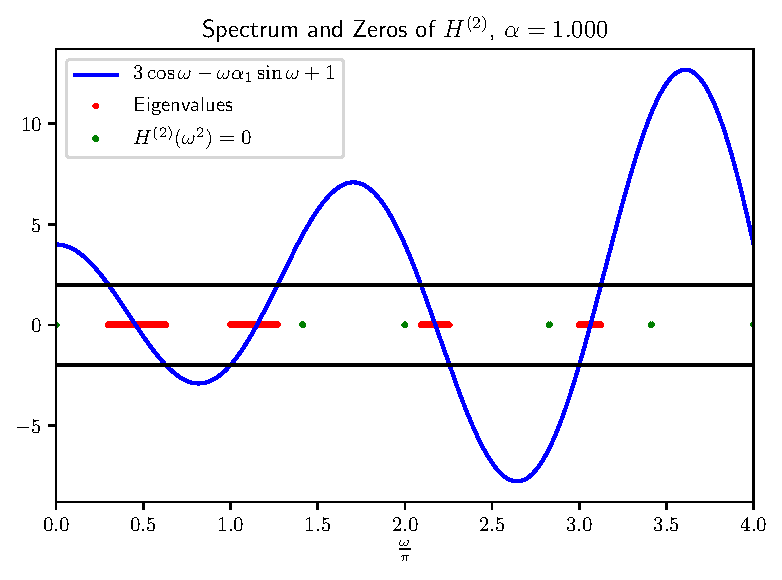
\includegraphics[scale=0.55]{1DDecoratedGraph_alpha1.pdf}
		\caption{\label{fig:1DDecoratedGraph_alpha1} The values of $\omega$ which solve \eqref{eq:EmbeddedGraphDetSolveCondition} with $\alpha_1=1$. No zeros of $H^{(2)}$ form part of the spectrum in this case.}
	\end{subfigure}
	~
	\begin{subfigure}[t]{0.45\textwidth}
		\centering
		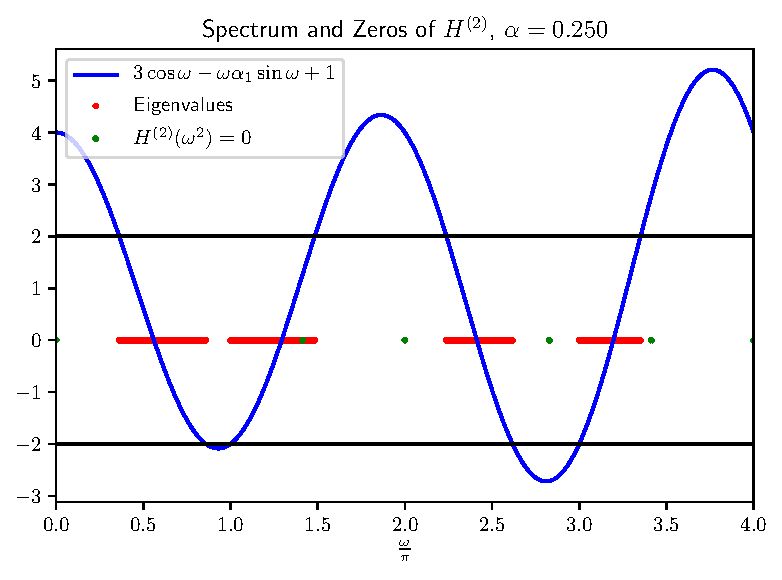
\includegraphics[scale=0.55]{1DDecoratedGraph_alpha0-25.pdf}
		\caption{\label{fig:1DDecoratedGraph_alpha0-25} The values of $\omega$ which solve \eqref{eq:EmbeddedGraphDetSolveCondition} with $\alpha_1=\recip{4}$. With $\alpha_1$ this small, some of the zeros of $H^{(2)}$ form part of the spectrum.}
	\end{subfigure}
	\caption{\label{fig:1DDecoratedGraph} The values of $\omega$ which solve \eqref{eq:EmbeddedGraphDetSolveCondition}, using $a=\recip{\sqrt{2}}$. Changing the value of $\alpha$ effects how many zeros of $H^{(2)}$ are included in the spectrum.}
\end{figure}
Zeros of $H^{(2)}$ occur at $\omega= 2n\pi, \frac{n\pi}{a}, \frac{n\pi}{b}$, which also solve \eqref{eq:EmbeddedGraphDetSolveCondition} for all values of $\qm$.
Examining the limit \eqref{eq:EigenvalueBranchLimit} reveals that if $H^{(2)}\bracs{\omega_0^2}=0$, $\omega_0$ is part of the spectrum only when there exists a $\qm_0\in\left[-\pi,\pi\right)$ such that $\Xi\bracs{\omega_0}=\cos\theta_0+\recip{2}$.
That is, the bracketed term in \eqref{eq:EmbeddedGraphDetSolveCondition} is required to be zero for a root of $H^{(2)}$ to be part of the spectrum.
The eigenvalue branches in the vicinity of root $\omega_0=\pi\sqrt{2}$ are plotted in figure \ref{fig:1DDecoratedGraphEvalBranches-Thetas}, to illustrate this point.
\begin{figure}[t!]
	\centering
	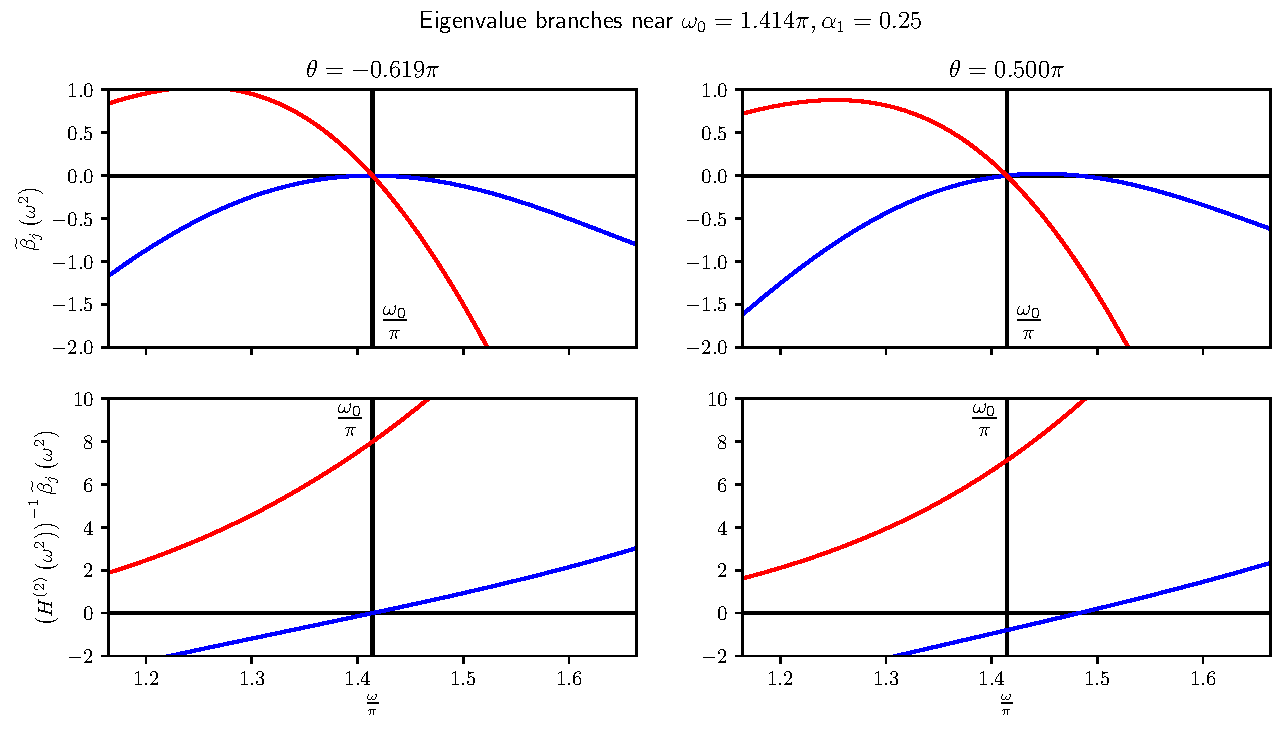
\includegraphics[scale=0.7]{1DDecoratedGraphEvalBranches-Thetas.pdf}
	\caption{\label{fig:1DDecoratedGraphEvalBranches-Thetas} eigenvalue branches of the matrix $\mathfrak{M}_{\qm}$ near $\omega_0 = \pi\sqrt{2}$, which is a root of $H^{(2)}$. The value $\qm_0\approx-0.691\pi$ solves $\Xi\bracs{\omega_0}=\cos\qm_0+\recip{2}$, and the limit \eqref{eq:EigenvalueBranchLimit} is zero. At other values of $\qm$ however, the limit \eqref{eq:EigenvalueBranchLimit} is non-zero.}
\end{figure}
It is also worth noting that (in figure \ref{fig:1DDecoratedGraphEvalBranches-Thetas}) there are two eigenvalue branches which are zero at $\omega_0$, with the third being non-zero at $\omega_0$.
For both branches, the limit \eqref{eq:EigenvalueBranchLimit} exists, however only for one is it zero.
The spectrum of \eqref{eq:WholeSpaceLaplaceEqn} thus consists of those $\omega$ such that
\begin{align*}
	\abs{ 3\cos\omega - \alpha_1\omega\sin\omega + 1 } \leq 2.
\end{align*}
As expected, the spectrum does not depend on $\beta$ despite the fact that the $M$-matrix for each operator on $\graph_{\mathcal{P}}$ does.
It does differ from the spectrum of the quantum graph in section \ref{ssec:Example1DLoop} due to the presence of the ``decoration" $I_{12}$, although this difference only depends on the length this additional edge.

\subsection{Cross in the Periodic Plane} \label{ssec:ExampleCrossInPlane}
Our final example is a two-dimensional graph whose period cell represents a lattice-like structure in $\reals^2$.
Consider the embedded, periodic graph defined as follows --- for each $\bracs{n,m}\in\integers^2$ define
\begin{align*}
	v^{(n,m)} &= \bracs{n+\recip{2}, m+\recip{2}}, \quad
	I_{\mathrm{left}}^{\bracs{n,m}} = \sqbracs{v^{\bracs{n,m}}, v^{\bracs{n+1,m}}}, \quad
	I_{\mathrm{up}}^{\bracs{n,m}} = \sqbracs{v^{\bracs{n,m}}, v^{\bracs{n,m+1}}}, \\
	\vertSet^* &= \clbracs{v^{\bracs{n,m}} \setVert \bracs{n,m}\in\integers^2}, \quad
	\edgeSet^* = \clbracs{ I_{\mathrm{l}}^{\bracs{n,m}}, I_{\mathrm{u}}^{\bracs{n,m}} \setVert \bracs{n,m}\in\integers^2}, \quad
	\graph^* = \bracs{\vertSet^*, \edgeSet^*}.
\end{align*}
Place a coupling constant $\alpha^{\bracs{n,m}} =: \alpha_3>0$ at each $v^{(n,m)}$.
The period graph of $\graph^*$ occupies $\left[0,1\right)^2$ and consists of a single vertex with two looping edges of length 1.
Breaking the loops by introducing two artificial vertices takes us to the quantum graph
\begin{align*}
	\vertSet = \clbracs{v_1, v_2, v_3}, \quad
	\edgeSet = \clbracs{I_{13}, I_{31}, I_{23}, I_{32}}, \quad
	\graph = \bracs{\vertSet, \edgeSet},
\end{align*}
with
\begin{align*}
	l_{13} = b, \quad l_{31} = \tilde{b} := 1-b, \quad 
	l_{23} = a, \quad l_{32} = \tilde{a} := 1-a, \qquad
	\qm_{13} = \qm_{31} = \qm_2, \quad \qm_{23} = \qm_{32} = \qm_1,
\end{align*}
and coupling constant $\alpha_3$ at $v_3$ (and zero coupling constants at the dummy vertices $v_1$ and $v_2$).
Also define
\begin{alignat*}{4}
	 s_a\bracs{\omega} &= \sin\bracs{a\omega}, \quad 
	 & c_a\bracs{\omega} = \cos\bracs{a\omega}, \quad 
	 s_b\bracs{\omega} &= \sin\bracs{b\omega}, \quad 
	 & c_b\bracs{\omega} = \cos\bracs{b\omega}, \\
	 \tilde{s}_a\bracs{\omega} &= \sin\bracs{\omega\bracs{1-a}}, \quad 
	 \tilde{c}_a\bracs{\omega} &= \cos\bracs{\omega\bracs{1-a}}, \quad 
	 \tilde{s}_b\bracs{\omega} &= \sin\bracs{\omega\bracs{1-b}}, \quad 
	 \tilde{c}_b\bracs{\omega} &= \cos\bracs{\omega\bracs{1-b}}.
\end{alignat*}
Using corollary \ref{cory:M-MatrixEntriesNoPoles} we set $H^{(2)}\bracs{\omega^2} = s_a\bracs{\omega} s_b\bracs{\omega} \tilde{s}_a\bracs{\omega} \tilde{s}_b\bracs{\omega}$, and obtain
\begin{align*}
	\mathfrak{M}_{\qm}\bracs{\omega^2} &=
	\begin{pmatrix}[2.5]
		-\omega s_a \tilde{s}_a \bracs{ s_b \tilde{c}_b + c_b \tilde{s}_b } &
		0 &
		\begin{split}
			&\omega s_a \tilde{s}_a \bracs{ e^{\rmi\qm_2\tilde{b}}s_b + e^{-\rmi\qm_2 b}\tilde{s}_b }
		\end{split} \\
		0 &
		-\omega s_b \tilde{s}_b \bracs{ s_a \tilde{c}_a + c_a \tilde{s}_a } &
		\begin{split}
			&\omega s_b \tilde{s}_b \bracs{ e^{\rmi\qm_1\tilde{a}}s_a + e^{-\rmi\qm_1 a}\tilde{s}_a } 
		\end{split} \\
		\omega s_a \tilde{s}_a \bracs{ e^{-\rmi\qm_2\tilde{b})}s_b + e^{\rmi\qm_2 b}\tilde{s}_b } &
		\omega s_b \tilde{s}_b \bracs{ e^{-\rmi\qm_1\tilde{a}}s_a + e^{\rmi\qm_1 a}\tilde{s}_a } &
		\begin{split}
			&-\omega ( s_a s_b \tilde{s}_a \tilde{c}_b 
			+ s_a s_b \tilde{c}_a \tilde{s}_b \\ 
			& + s_a c_b \tilde{s}_a \tilde{s}_b
			+ c_a s_b \tilde{s}_a \tilde{s}_b \\
			& - \omega\alpha_3 s_a s_b \tilde{s}_a \tilde{s}_b )
		\end{split}
	\end{pmatrix}.
\end{align*}
Examining \eqref{eq:QGDetSolveCondition} yields
\begin{align} \label{eq:ExampleThickVertexSolution}
	0 = \omega^3 s_a^2\bracs{\omega} s_b^2\bracs{\omega} \tilde{s}_a^2\bracs{\omega} \tilde{s}_b^2\bracs{\omega} \sin\bracs{\omega} 
	\bracs{ 4\cos\bracs{\frac{\qm_1+\qm_2}{2}}\cos\bracs{\frac{\qm_1-\qm_2}{2}} + \omega\alpha_3\sin\omega - 4\cos\omega}.
\end{align}
For ease, we define
\begin{align*}
	\Xi\bracs{\omega} := \cos\omega - \frac{\alpha_3\omega}{4}\sin\omega.
\end{align*}
From here, the analysis is similar to that of example \ref{ssec:EmbeddingDependentExample} --- any root of $H^{(2)}$ solves \eqref{eq:ExampleThickVertexSolution}, in addition to those $\omega$ for which $-1\leq\Xi\bracs{\omega}\leq 1$.
Examination of the eigenvalue branches then produces a familiar conclusion; if $H^{(2)}\bracs{\omega_0^2}=0$, $\omega_0$ forms part of the spectrum of \eqref{eq:QGFullSystem} on $\graph$ if and only if there exists a $\qm_0$ such that the bracket in \eqref{eq:ExampleThickVertexSolution} is zero at $\bracs{\omega_0,\qm_0}$ -- that is if $\Xi\bracs{\omega_0} = \cos\bracs{\frac{\bracs{\qm_0}_1+\bracs{\qm_0}_2}{2}}\cos\bracs{\frac{\bracs{\qm_0}_1-\bracs{\qm_0}_2}{2}}$.
As a result, the spectrum consists of exactly those $\omega$ such that
\begin{align*}
	-1 \leq \cos\omega - \frac{\alpha_3\omega}{4}\sin\omega \leq 1.
\end{align*}
To round off the analysis, quantities such as the integrated density of states (IDoS) and density of states (DoS) can also be estimated from \eqref{eq:ExampleThickVertexSolution}, which demonstrating that the spectrum ``concentrates" at the center of each spectral band.
Examples are shown in figure \ref{fig:CrossInPlane_ScalarDoS}.
\begin{figure}[b!]
	\begin{subfigure}[t]{0.45\textwidth}
		\centering
		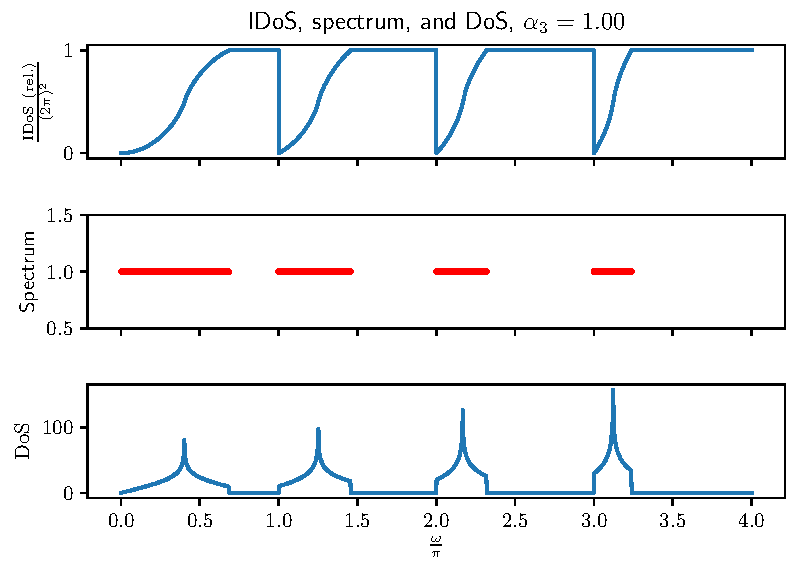
\includegraphics[scale=0.5]{CrossInPlane_ScalarDoS_alpha1-00.pdf}
		\caption{\label{fig:CrossInPlane_ScalarDoS_alpha1-00} The (relative) integrated density of states (IDoS), density of states (DoS) and spectrum for the system with $\alpha_3=1$.}
	\end{subfigure}
	~
	\begin{subfigure}[t]{0.45\textwidth}
		\centering
		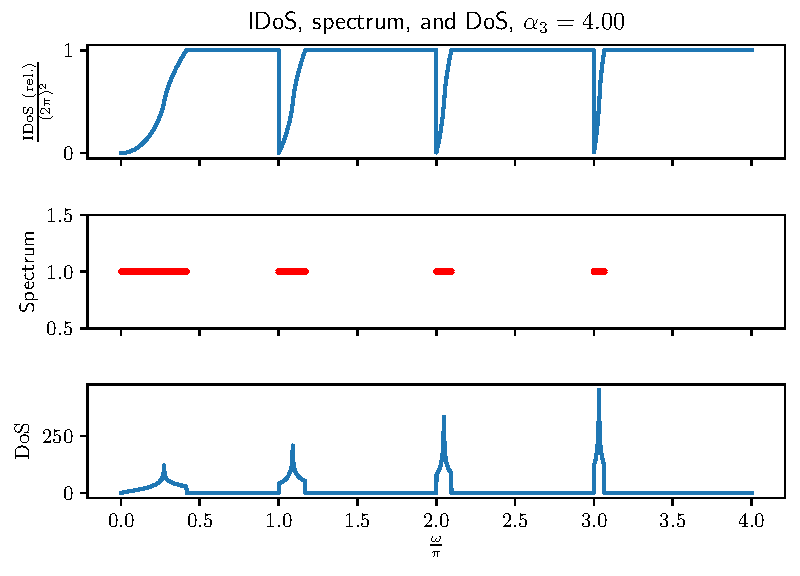
\includegraphics[scale=0.5]{CrossInPlane_ScalarDoS_alpha4-00.pdf}
		\caption{\label{fig:CrossInPlane_ScalarDoS_alpha4-00} The (relative) integrated density of states (IDoS), density of states (DoS) and spectrum for the system with $\alpha_3=4$.}
	\end{subfigure}	
	\caption{\label{fig:CrossInPlane_ScalarDoS} The (relative) IDoS, DoS, and spectrum for the graph topology in section \ref{ssec:ExampleCrossInPlane}.
	The relative IDoS at the value $x$ is defined as the IDoS at the value $x$ minus $\left\lfloor\frac{x}{\pi}\right\rfloor\bracs{2\pi}^2$.}
\end{figure}
For any $\alpha_3>0$, the spectrum comprises a union of pairwise disjoint ``spectral bands" $I_n\subset\sqbracs{(n-1)\pi, n\pi}$, each with left-endpoint $(n-1)\pi$ and a right-endpoint strictly less than $n\pi$.
It is worth remarking that this behaviour is reversed for $\alpha_3<0$, the bands having right-endpoint $n\pi$ and left-endpoint strictly greater than $(n-1)\pi$.
For $\alpha\leq-2$ there is even a gap between an isolated eigenvalue at $0$ and the beginning of the band $I_1$ --- however as mentioned in section \ref{ssec:PhysMot}, $\alpha<0$ has no physical basis.
This is consistent with similar applications of singular-structures as approximations to thin-material structures, like the work of \cite{cherednichenko2019time}, in which the natural physical constraints on the parameters in the problem prevent the opening of a band-gap at the bottom of the spectrum.
